\documentclass{article}

\title{The Impact of Police Violence on Confidence in Institutions}
\date{October 24, 2017}
\author{Matthew Harvey}
\usepackage{amsmath}
\usepackage{graphicx}
\usepackage{booktabs}

\begin{document}
  \maketitle
  
\section{ Motivation and Relevant Literature}

\paragraph{}While there have been numerous studies in economics and other social sciences that have examined the determinants of police violence, there has been no examination of its effects. In his paper on police use of force, Roland Fryer finds that police officers use non-lethal force more often on minorities; however, this differential use of force toward minorities ceases when force turns deadly \cite{fryer2016empirical}. Other studies in sociology have examined the determinants of deadly police force \cite{jacobs1998determinants} \cite{jacobs1979inequality}, yet I have seen no studies within economics or other fields that look at the effects of police violence. Although there have been precious few studies on the effects of police violence, Alsan and Wanamaker's analysis of the effects of the illicit Tuskegee syphilis experiment \cite{alsan2016tuskegee}. They show that years after the illicit experiment, black men in the area still distrusted health professionals while trust levels for other races near the experiment remained nearly the same. 
\paragraph{} Others have examine police violence and fatalities as an outcome, but I elect to use police violence as an explanatory variable to account for the variation in confidence in institutions. Similar to Alsan's method, I intend to use a difference in difference analysis between races before and after a particular police fatality to determine its effect on an individuals confidence in institutions. Based on Alsan findings, the effects on trust will be stronger for fatalities close to an individual and where the individual can identify with the victim \cite{alsan2016tuskegee}. However, as this Tuskegee experiment occurred before the advent of the Internet, one could expect different results. Alsan's findings hinged partially on the dissemination of information to those in close proximity to the study. Reactions to police induced fatalities could be more widespread due to the ease of access to information and the rise of social media \footnote{It is very likely that those who would have no knowledge of a particular event could find out through friends much more easily due to the advent of the Internet}.  As more salient instances are also more likely to attract attention, I also intend to add another variable to this data that will capture the salience of a particular fatality \footnote{To do this I will either look use Lexus Nexus or look at the Fatal Encounters' attach article and determine how many views it received}.

\section{The Data and Summary Statistics}

\subsection{Fatal Encounters: The Police Induced Fatality Data}

\paragraph{}The data I propose to use is a combination of data sets from the website Fatal Encounters which is a data set of all police induced fatalities since $2000$ with information on the location of the fatality, the victim's demographic information (particularly the victim's race), and the department involved with the fatality.  Below I give a two summary representations of the data: the first is the number of police fatalities by year and the second is the number of police fatalities by race. I forgo any spatial representation of the data solely because my analysis will be forced to pool observations for different fatalities \footnote{For example, a shooting that occurs in Flagstaff cannot be counted as a single event, rather for a given time frame, I will have to create a proximity to a police fatality variable. This is because of the relatively low number of observations in the Gallup data. The Gallup data also only has individuals' geographic information at the city level.}


\begin{figure}[h!]
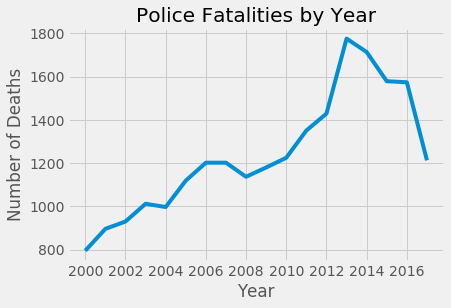
\includegraphics[width=75mm,scale=0.1]{DeathToll.png}
\centering
\caption{}
\end{figure}

The above graph tracks police induced fatalities for all races by year. It is interesting to note that until $2013$ there seemed to be an upward trend in police induced fatalities. It would seem that after $2013$ the number of police induced deaths declined, although one cannot be certain of this trend as the data for $2017$ is not complete. While such a representation is not necessary for a difference in difference analysis, it can show what years one should use for the two sets of cross-sectional data. Here police fatalities spike between $2012$ and $2013$ which would mean if one expects an effect based on volume of shootings, these would be the years to examine. 

\paragraph{}Figure two displays the number of police induced fatalities by race. 

\begin{figure}[h!]
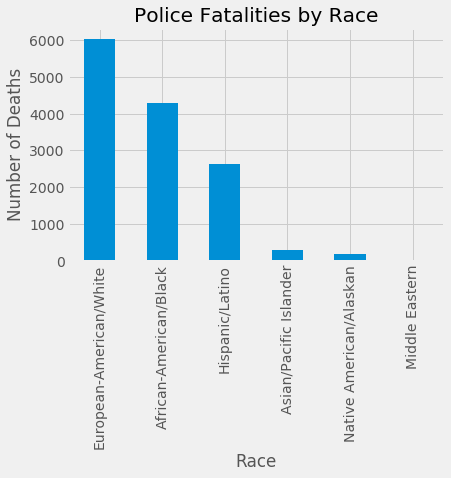
\includegraphics[width=75mm,scale=0.1]{Race.png}
\centering
\caption{}
\end{figure}

It would seems that there are more minority deaths at the hands of police relative to their respective population weights. However, this graph fails to control for other factors like socioeconomic status, whether or not the victim was armed, or the victim's criminal history all of which could lead to a different result. 

\pagebreak

\subsection{Gallup Confidence in Institutions Poll: The Proxy For Trust}

My analysis will merge the above data set with information from Gallup's \textit{Confidence in Institutions} survey. This data stretches from $1973$ to $2016$. Since this data begins far before the fatality data, I will be able to examine the parallel trends assumption without any loss of observations. The one caveat of this data set is that that it only contains about $1,000$ observations per year despite its rich information for each observation. The subsequent figure displays the number of respondents of each race in the data set.

\pagebreak

\begin{figure}[h!]
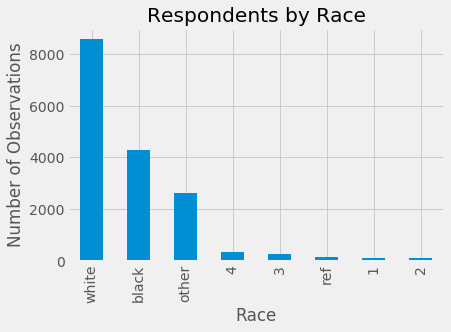
\includegraphics[width=75mm,scale=0.1]{Race_Respondents.png}
\centering
\caption{}
\end{figure}

This figure present what may be a potential problem with our identification strategy. Despite the large numbers of Black and Hispanic victims of police fatalities, the respondent data set is much more heavily white. This does not necessarily pose a problem for the overall research question; however, the low number of minority respondents could make it difficult to find any effect for   police induced fatalities on minority confidence in institutions. This also means that if there is a negative effect, it is likely biased downwards since one would expect that minorities would have a more negative reaction to institutions as a result of police induced fatalities.  

\section{Preliminary Regressions}

\paragraph{}Here I begin to run preliminary logistic regressions to see whether or not police violence affects the confidence in institutions. I take the data from both \textit{Gallup} and \textit{Fatal Encounters} and combine by year and zip code. In other words, the variable $Death_{i}$ is a dummy equal to one if there is a police induced death in a given zip code in a given year. The first specification regresses a dummy for whether the police are fair to blacks or not on a host of covariates.

\subsection{Model I: The Basic Logit with Police Fairness}

\begin{tabular}{lclc}
\toprule
\textbf{Dep. Variable:} & Unfair\_2\_Blacks  & \textbf{  No. Observations:  } &      1408    \\
\textbf{Model:}         &      Logit       & \textbf{  Df Residuals:      } &      1404    \\
\textbf{Method:}        &       MLE        & \textbf{  Df Model:          } &         3    \\
\textbf{Date:}          & Tue, 31 Oct 2017 & \textbf{  Pseudo R-squ.:     } &      -inf    \\
\textbf{Time:}          &     10:40:48     & \textbf{  Log-Likelihood:    } &       -inf   \\
\textbf{converged:}     &      False       & \textbf{  LL-Null:           } & -3.5457e+05  \\
\bottomrule
\end{tabular}
\begin{tabular}{lcccccc}
               & \textbf{coef} & \textbf{std err} & \textbf{z} & \textbf{$P>|z|$} & \textbf{[0.025} & \textbf{0.975]}  \\
\midrule
\textbf{Death} &      -7.5301  &        1.041     &    -7.234  &         0.000        &       -9.570    &       -5.490     \\
\textbf{age}   &       0.0255  &        0.005     &     4.648  &         0.000        &        0.015    &        0.036     \\
\textbf{black} &       6.9219  &        1.006     &     6.879  &         0.000        &        4.950    &        8.894     \\
\textbf{white} &     -25.8350  &     4.15e+05     & -6.23e-05  &         1.000        &    -8.13e+05    &     8.13e+05     \\
\bottomrule
\end{tabular}
%\caption{Logit Regression Results}

\bigskip

Here we see that the $Death_{i}$ variable is negative and statistically significant, indicating that a police induced death in one's area makes one less likely to think that blacks are receiving unfair treatment from the police. It is worth noting, however, that the dummy variable for a Black survey respondent is both positive and significant. This means that there may be a differential effect on death based on race (the white dummy variable is also negative, but insignificant) \footnote{In further regressions, I will interact the  $Death_{i}$ and Black variables to parse out this effect.}.

\subsection{Model II: Additional Covariates for Dwelling Status}
In the second specification, I add dummy variables for whether one lives in a urban ($city_{i}$), suburban ($suburbia_{i}$), or rural ($rural_{i}$) region. 

\bigskip

\begin{tabular}{lclc}
\toprule
\textbf{Dep. Variable:} & Unfair\_2\_Blacks  & \textbf{  No. Observations:  } &      1408    \\
\textbf{Model:}         &      Logit       & \textbf{  Df Residuals:      } &      1402    \\
\textbf{Method:}        &       MLE        & \textbf{  Df Model:          } &         5    \\
\textbf{Date:}          & Tue, 31 Oct 2017 & \textbf{  Pseudo R-squ.:     } &      -inf    \\
\textbf{Time:}          &     11:29:14     & \textbf{  Log-Likelihood:    } &       -inf   \\
\textbf{converged:}     &       True       & \textbf{  LL-Null:           } & -3.5457e+05  \\
\bottomrule
\end{tabular}
\begin{tabular}{lcccccc}
                  & \textbf{coef} & \textbf{std err} & \textbf{z} & \textbf{P$>$$|$z$|$} & \textbf{[0.025} & \textbf{0.975]}  \\
\midrule
\textbf{Death}    &      -7.8091  &        1.061     &    -7.359  &         0.000        &       -9.889    &       -5.729     \\
\textbf{age}      &       0.0227  &        0.006     &     3.667  &         0.000        &        0.011    &        0.035     \\
\textbf{black}    &       8.0715  &        1.011     &     7.983  &         0.000        &        6.090    &       10.053     \\
\textbf{rural}    &      -1.6250  &        0.927     &    -1.753  &         0.080        &       -3.442    &        0.192     \\
\textbf{city}     &      -2.1273  &        0.264     &    -8.058  &         0.000        &       -2.645    &       -1.610     \\
\textbf{suburbia} &      -4.5509  &        1.037     &    -4.387  &         0.000        &       -6.584    &       -2.518     \\
\bottomrule
\end{tabular}
%\caption{Logit Regression Results}

\bigskip

Here we see that the coefficient on the $Death_{i}$ variable does not change much in either magnitude or significance. We also see the that the population/dwelling controls seem to soak up some of the variation as they are all significant \footnote{The $rural_{i}$ variable is only significant at the $90\%$ confidence level, though.}. 

\subsection{Model III: Racial Relations}

The final model explores whether or not the $Death_{i}$ variable has any effect on ideas about the future of race relations. I also add the base level covariates I have added to all the other models (age and race).

\begin{tabular}{lclc}
\toprule
\textbf{Dep. Variable:} & problem\_forever  & \textbf{  No. Observations:  } &     1408    \\
\textbf{Model:}         &      Logit       & \textbf{  Df Residuals:      } &     1404    \\
\textbf{Method:}        &       MLE        & \textbf{  Df Model:          } &        3    \\
\textbf{Date:}          & Tue, 31 Oct 2017 & \textbf{  Pseudo R-squ.:     } &  -0.06403   \\
\textbf{Time:}          &     10:40:48     & \textbf{  Log-Likelihood:    } &   -99218.   \\
\textbf{converged:}     &       True       & \textbf{  LL-Null:           } &   -93247.   \\
\bottomrule
\end{tabular}
\begin{tabular}{lcccccc}
               & \textbf{coef} & \textbf{std err} & \textbf{z} & \textbf{P$>$$|$z$|$} & \textbf{[0.025} & \textbf{0.975]}  \\
\midrule
\textbf{Death} &      -0.6163  &        0.159     &    -3.878  &         0.000        &       -0.928    &       -0.305     \\
\textbf{age}   &       0.0009  &        0.003     &     0.306  &         0.760        &       -0.005    &        0.007     \\
\textbf{black} &       0.4701  &        0.130     &     3.605  &         0.000        &        0.215    &        0.726     \\
\textbf{white} &      -0.0640  &        0.144     &    -0.444  &         0.657        &       -0.346    &        0.218     \\
\bottomrule
\end{tabular}
%\caption{Logit Regression Results}

\bigskip

The results show that a police induced death in ones area actually decreases one's likelihood to believe that blacks and whites have issues that will never be resolved. Here we once again see that the impact is differential between races (though still insignificant for whites). This provides more evidence that the potentially chief interesting question of this work going forward is to examine the effects of police induced deaths differentially by race.

\pagebreak

\bibliographystyle{plain}
\bibliography{Econ880_Police_Bib}

\end{document}